% !TEX TS-program = XeLaTeX
% use the following command:
% all document files must be coded in UTF-8
\documentclass[portuguese]{textolivre}
% build HTML with: make4ht -e build.lua -c textolivre.cfg -x -u article "fn-in,svg,pic-align"
\usepackage{graphicx}
\usepackage{subcaption}

\journalname{Texto Livre}
\thevolume{18}
%\thenumber{1} % old template
\theyear{2025}
\receiveddate{\DTMdisplaydate{2025}{1}{13}{-1}} % YYYY MM DD
\accepteddate{\DTMdisplaydate{2025}{2}{17}{-1}}
\publisheddate{\DTMdisplaydate{2025}{7}{14}{-1}}
\corrauthor{Tiago Giuriatti}
\articledoi{10.1590/1983-3652.2025.56958}
%\articleid{NNNN} % if the article ID is not the last 5 numbers of its DOI, provide it using \articleid{} commmand 
% list of available sesscions in the journal: articles, dossier, reports, essays, reviews, interviews, editorial
\articlesessionname{articles}
\runningauthor{Giuriatti et al.} 
%\editorname{Leonardo Araújo} % old template
\sectioneditorname{Daniervelin Pereira}
\layouteditorname{Saula Cecília}

\title{Cognição universitária: \textit{framework} para infraestrutura de um \textit{campus}}
\othertitle{University cognition: framework for campus infrastructure}
% if there is a third language title, add here:
%\othertitle{Artikelvorlage zur Einreichung beim Texto Livre Journal}

\author[1]{Tiago Giuriatti~\orcid{0000-0001-6998-2442}\thanks{Email: \href{mailto:giuriatti1989@gmail.com}{giuriatti1989@gmail.com}}}
\author[1]{João Artur de Souza~\orcid{0000-0002-7133-8944}\thanks{Email: \href{mailto:joao.artur@ufsc.br}{joao.artur@ufsc.br}}}
\author[1]{Gilberto Luiz de Souza Paula~\orcid{0000-0001-9945-2856}\thanks{Email: \href{mailto:gilbertoluizfisico@gmail.com}{gilbertoluizfisico@gmail.com}}}
\author[2]{Chirley de Miranda Giuriatti~\orcid{0009-0007-5977-6291}\thanks{Email: \href{mailto:chirleymiranda@gmail.com}{chirleymiranda@gmail.com}}}
\affil[1]{Universidade Federal de Santa Catarina,  Programa de Pós-Graduação e Engenharia de Conhecimento, Florianópolis, SC, Brasil.}
\affil[2]{Instituto Federal Catarinense, Blumenau, SC, Brasil.}

\addbibresource{article.bib}
% use biber instead of bibtex
% $ biber article

% used to create dummy text for the template file
\definecolor{dark-gray}{gray}{0.35} % color used to display dummy texts
\usepackage{lipsum}
\SetLipsumParListSurrounders{\colorlet{oldcolor}{.}\color{dark-gray}}{\color{oldcolor}}

% used here only to provide the XeLaTeX and BibTeX logos
\usepackage{hologo}

% if you use multirows in a table, include the multirow package
\usepackage{multirow}

% provides sidewaysfigure environment
\usepackage{rotating}

% CUSTOM EPIGRAPH - BEGIN 
%%% https://tex.stackexchange.com/questions/193178/specific-epigraph-style
\usepackage{epigraph}
\renewcommand\textflush{flushright}
\makeatletter
\newlength\epitextskip
\pretocmd{\@epitext}{\em}{}{}
\apptocmd{\@epitext}{\em}{}{}
\patchcmd{\epigraph}{\@epitext{#1}\\}{\@epitext{#1}\\[\epitextskip]}{}{}
\makeatother
\setlength\epigraphrule{0pt}
\setlength\epitextskip{0.5ex}
\setlength\epigraphwidth{.7\textwidth}
% CUSTOM EPIGRAPH - END

% to use IPA symbols in unicode add
%\usepackage{fontspec}
%\newfontfamily\ipafont{CMU Serif}
%\newcommand{\ipa}[1]{{\ipafont #1}}
% and in the text you may use the \ipa{...} command passing the symbols in unicode

% LANGUAGE - BEGIN
% ARABIC
% for languages that use special fonts, you must provide the typeface that will be used
% \setotherlanguage{arabic}
% \newfontfamily\arabicfont[Script=Arabic]{Amiri}
% \newfontfamily\arabicfontsf[Script=Arabic]{Amiri}
% \newfontfamily\arabicfonttt[Script=Arabic]{Amiri}
%
% in the article, to add arabic text use: \textlang{arabic}{ ... }
%
% RUSSIAN
% for russian text we also need to define fonts with support for Cyrillic script
% \usepackage{fontspec}
% \setotherlanguage{russian}
% \newfontfamily\cyrillicfont{Times New Roman}
% \newfontfamily\cyrillicfontsf{Times New Roman}[Script=Cyrillic]
% \newfontfamily\cyrillicfonttt{Times New Roman}[Script=Cyrillic]
%
% in the text use \begin{russian} ... \end{russian}
% LANGUAGE - END

% EMOJIS - BEGIN
% to use emoticons in your manuscript
% https://stackoverflow.com/questions/190145/how-to-insert-emoticons-in-latex/57076064
% using font Symbola, which has full support
% the font may be downloaded at:
% https://dn-works.com/ufas/
% add to preamble:
% \newfontfamily\Symbola{Symbola}
% in the text use:
% {\Symbola }
% EMOJIS - END

% LABEL REFERENCE TO DESCRIPTIVE LIST - BEGIN
% reference itens in a descriptive list using their labels instead of numbers
% insert the code below in the preambule:
%\makeatletter
%\let\orgdescriptionlabel\descriptionlabel
%\renewcommand*{\descriptionlabel}[1]{%
%  \let\orglabel\label
%  \let\label\@gobble
%  \phantomsection
%  \edef\@currentlabel{#1\unskip}%
%  \let\label\orglabel
%  \orgdescriptionlabel{#1}%
%}
%\makeatother
%
% in your document, use as illustraded here:
%\begin{description}
%  \item[first\label{itm1}] this is only an example;
%  % ...  add more items
%\end{description}
% LABEL REFERENCE TO DESCRIPTIVE LIST - END


% add line numbers for submission
%\usepackage{lineno}
%\linenumbers

\begin{document}
\maketitle

\begin{polyabstract}
\begin{abstract}
Na busca da literatura atual, encontra-se a evolução do conceito \textit{smart} para o cognitivo no contexto universitário. Estruturas \textit{smart} foram desenvolvidas por autores em domínios e respectivas dimensões. No entanto, no contexto da cognição, o ambiente universitário na literatura, demonstra somente modelos com aplicações em campos específicos, sem, contudo, a definição de uma estrutura para esses ambientes. Nesse sentido, o objetivo e pergunta de pesquisa envolve ``como estruturar um \textit{framework} para um campus universitário transformando-o em cognitivo?". A estrutura considera elementos referentes à revisão teórica dos artigos pelas dimensões, termos e atributos dos modelos cognitivos aplicados no ambiente universitário na dimensão infraestrutura. Também absorve os resultados da revisão da literatura dos modelos \textit{smart campus} e da estrutura dos modelos cognitivos no contexto das cidades, por serem uma amplificação do ambiente de um campus em escala maior. A estrutura é validada por uma ontologia na ferramenta Protégé, sendo traçados cinco domínios, classificados por classes e as respectivas métricas com suas instâncias. Os resultados demonstram um \textit{framework} nos domínios Pessoas, Ambiente e Áreas Construídas, Uso do Espaço, Uso dos Recursos Tecnológicos e Governança. Tornando-se aderentes ao contexto universitário para a cognição, sendo as ferramentas com maior relevância nestes domínios os sensores, receptores e IA; agentes responsáveis pela captação, distribuição, armazenamento e transformação dos dados em resposta às demandas contidas nas ontologias definidas pelas subclasses e instâncias.

\keywords{Ontologias\sep Domínios\sep Ferramentas\sep Cognição\sep Infraestrutura Universitária}
\end{abstract}

\begin{english}
\begin{abstract}
In the search for current literature, one finds the evolution of the smart concept to the cognitive one in the university context. Smart structures were developed by authors across domains and respective dimensions. However, in the context of cognition, which is an evolution of the smart concept for the university environment, the literature only demonstrates models with applications in specific fields, without, however, defining a structure for these environments. In this sense, the objective and research question involves ``how to structure a framework for a university campus so that its infrastructure makes it cognitive?". The structure considers elements relating to the theoretical review of articles by dimensions, terms and attributes of cognitive models applied in the university environment. It also absorbs the results of the literature review of smart campus models and the structure of cognitive models in the context of cities, as they are an amplification of the campus environment on a larger scale. The structure is validated by an ontology in the Protégé tool, with five domains being outlined, classified by classes and the respective metrics with their instances. The results demonstrate a structure validated by the ontology in the domains People, Environment and Built Areas, Use of Space, Use of Technological Resources and Governance that adhere to the university context for cognition, with the most relevant tools in these domains being sensors, receptors and AI; agents responsible for capturing, distributing, storing and transforming data in response to the demands contained in the ontologies defined by subclasses and instances.

\keywords{Ontologies\sep Domains\sep Tools\sep Cognition\sep University Infrastructure}
\end{abstract}
\end{english}
% if there is another abstract, insert it here using the same scheme
\end{polyabstract}

\section{Introdução}\label{sec-intro}
A disseminação de informações, bem como a colaboração, as trocas e o compartilhamento destas no meio interno e externo ao \textit{campus} podem ser aprimorados em um ambiente inteligente, \textit{``smart"}; o qual pode melhorar o aprendizado e desenvolvimento de habilidades, sendo o local em que se espera que os alunos possam compartilhar informações em qualquer lugar, a qualquer hora \cite{lessard2021}.

Um ambiente inteligente é aquele em que as ações de vários controladores em rede (controlando diferentes aspectos de um ambiente) são orquestradas por processos preventivos de autoprogramação (por exemplo, agentes de \textit{software} inteligentes) de forma a criar uma funcionalidade holística interativa que aprimora as experiências dos ocupantes \cite{augusto2013}(Augusto et al., 2013); são ambientes que conectam perfeitamente os sensores e telas para melhorar conhecimento do entorno e a qualidade de vida \cite{delorenzo2017}.

\textit{Smart Campus} é uma instância de um Ambiente Inteligente, criado para apoiar quem faz uso e interage com o \textit{campus} \cite{augusto2021}. Entendido como um ambiente aberto, inovador, colaborativo e integrado \cite{nobrega2021}, visa melhorar a gestão de todo o \textit{campus}, bem como atividades são desenvolvidas de forma inteligente \cite{musa2021}. Um dos bi-produtos das \textit{Smart Cities}, podendo ser dimensionado e adaptado a eles para criar um \textit{Smart Campus} \cite{pagliaro2016}; o campus inteligente é um ambiente de ensino, onde ocorre a interação dinâmica entre alunos/usuários e os dispositivos ao redor usando o paradigma da Internet das Coisas (IoT) \cite{hadwan2020}; aprimorando a educação, a pesquisa, o design e a entrega dos módulos de ensino superior apropriados para buscar os mais recentes desenvolvimentos em Tecnologias da Informação e Comunicação (TIC), que podem impulsionar o crescimento e a inovação educacional futura \cite{mustafa2021}.

Atualmente, os modelos \textit{smart campus} apoiam-se na ideia da interação usuário e campus, seja por sensores, ferramentas ou dispositivos baseados em IoT. Estes modelos buscam implementar e combinar no processo de ensino e aprendizagem ou em outras atividades acadêmicas do campus, ferramentas de tecnologia da informação como suporte para produzir serviços de campus inteligentes \cite{madyatmadja2021}; constatar uma localização no ambiente do usuário, identificar os serviços/locais mais próximos ao redor, além de guiar os usuários de sua localização para um local específico \cite{hadwan2020}; com disposição de sensores em banheiros na faculdade, como na Universidade Perlis Malaysia \cite{mansur2021}. Ou seja, os \textit{campi smart} são limitados a ações de resposta, sem um meio de gerenciar de forma resiliente e responsiva as demandas frente as mudanças constantes no ambiente.

Isso conduz à necessidade de promoção e desenvolvimento do conceito de \textit{campus} voltado à cognição, onde a universidade é um reator em que a geração de conhecimento, inovações e novos produtos é acelerada para além de um certo ponto crítico devido à concentração de inteligência, comunicação, atividade empreendedora e necessidade de recursos \cite{vasetskaya2020}. Uma vertente de campus cada vez mais conectado e responsivo as suas particularidades, levando a produzir, por exemplo:

\begin{itemize}
    \item i) Incremento e Intensificação do fluxo comunicativo-valorativo do conhecimento dentro da universidade e em sua interação com o ambiente externo;
    \item ii) Estímulos para os alunos dominarem o papel de gerente cognitivo, o que gera a produção de empreendedores inovadores a partir das competências cognitivas em estudantes universitários \cite{jimenez2019} e; 
    \item iii) Incentivos aos alunos para que desenvolvam suas meta-habilidades, que podem ser vistas como uma forma de resultados de gerenciamento cognitivo em instituições de ensino superior \cite{belyaev2019}.
\end{itemize}

A cognição pode ser categorizada por estilos cognitivos, como aqueles empregados por universidades Jordanianas que aplicam o estilo de conhecimento, estilo de planejamento e estilo de criação; sendo um ponto de inflexão na gestão contemporânea e de inovação estratégica de grande diferencial no valor agregado nestas universidades \cite{Alnazer2017}.

As universidades que buscam a cognição também empregam sistemas cognitivos baseados em computação cognitiva e aprendizado profundo \cite{golovianko2017}, além de sistemas cognitivos-generativos para formulação de um espaço criativo, sendo um gatilho motivador para a aprendizagem, criação de novos conhecimentos e sua aplicação socioeconômica \cite{karpov2018}.

A proposição de uma estrutura para a cognição no \textit{campus} visa atender as necessidades impostas atualmente pelo uso, interação e reutilização dos recursos no ambiente universitário. O \textit{campus} se torna um agente que sustenta suas ações para viabilizar, por exemplo, a sustentabilidade (base para aprendizagem no ambiente das cidades), consumo de energia e respostas dos edifícios do campus às variáveis internas e externas expostas nestes ambientes, como é o caso do campus proposto na ilha de Povelgia – Itália \cite{bittenbinder2020}, uma ampliação do modelo \textit{smart} promovido em Brescia, a primeira experiência no contexto italiano que integra o IBM Watson (agente cognitivo) como parte do conceito cognitivo.

A partir do estudo no contexto \textit{smart campus} por \textcite{giuriatti2023}, foi realizada a revisão da literatura sobre as dimensões que compreendem a customização universitária pelos domínios classificados, com destaque à questão de ambientes \textit{smart}, tecnologias \textit{smart}, infraestrutura \textit{smart}, aplicações \textit{smart}, sustentabilidade \textit{smart} e técnicas \textit{smart}; onde as TICs como IoT e Big Data possuem as maiores tendências.

A compreensão dos fatores que denotam o ambiente das cidades no contexto \textit{smart} facilita a identificação dos domínios e dimensões destas para o direcionamento no ambiente em menor escala, podendo ser caracterizado como o universitário \cite{ramlee2019, alrashed2020}, pois são laboratórios vivos para a inteligência futura das cidades globalmente \cite{omotayo2021}; como campo de testes para cidades inteligentes \cite{mohammadi2021}; ideais para construir e testar o modelo de cidade inteligente, devido ao contexto em que se inserem ser semelhante, principalmente as tecnologias e protocolos de comunicação compatíveis \cite{alrashed2020}. 

Para compreender o desenvolvimento do campus a partir dos modelos cognitivos nas cidades, pode-se correlacionar a aplicação pelo framework desenvolvido em várias dimensões \cite{giuriatti2024}.

%--- CÓDIGO DA FIGURA 1 ---%
% Primeira parte da figura
\begin{figure}[h!]
    \centering

    \begin{subfigure}[b]{\textwidth}
        \centering
        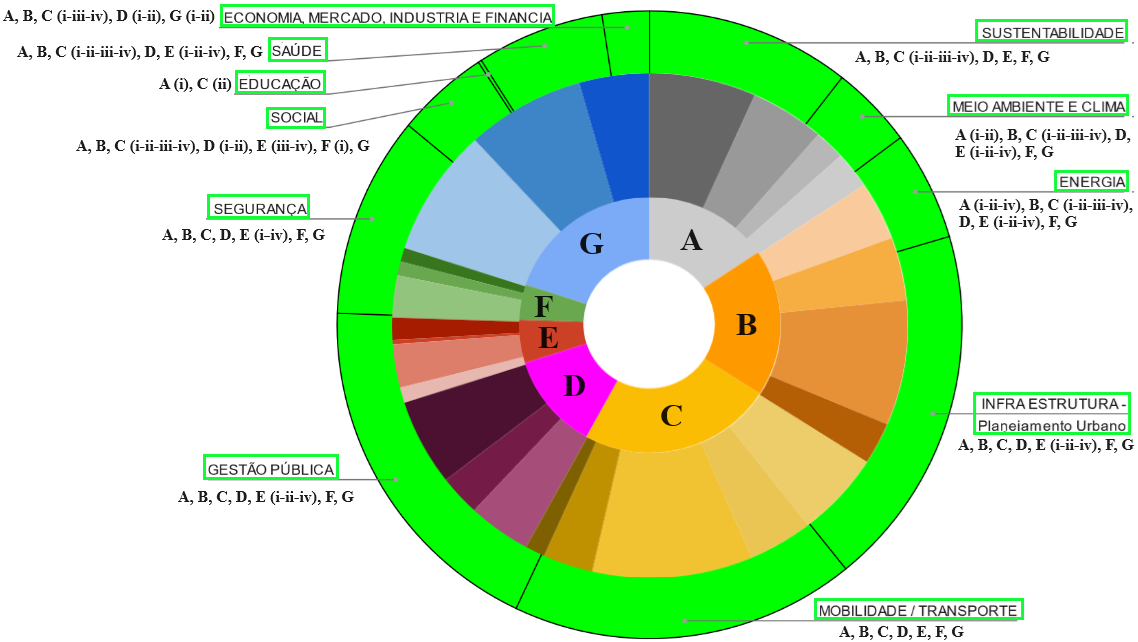
\includegraphics[width=0.9\textwidth,keepaspectratio]{images/FIGURA1_A.png}
        \caption{Estrutura do \textit{Framework}.}
        
    \end{subfigure}

    \vspace{0.5cm}

    \begin{subfigure}[b]{\textwidth}
        \centering
        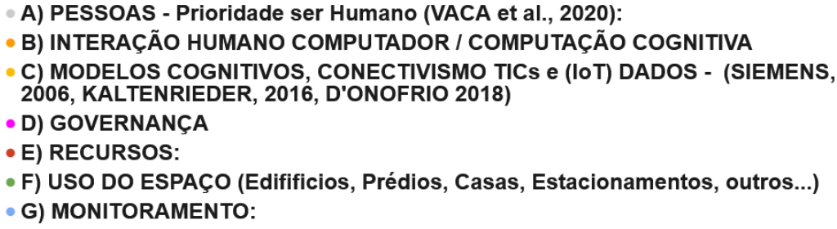
\includegraphics[width=0.75\textwidth,keepaspectratio]{images/FIGURA1_B.png}
        \caption{Domínios.}
        
    \end{subfigure}

\end{figure}

\clearpage

% Continuação da figura anterior
\begin{figure}[h!]
    \ContinuedFloat % <- importante: indica que é continuação da figura anterior
    \centering

    \begin{subfigure}[b]{\textwidth}
        \centering
        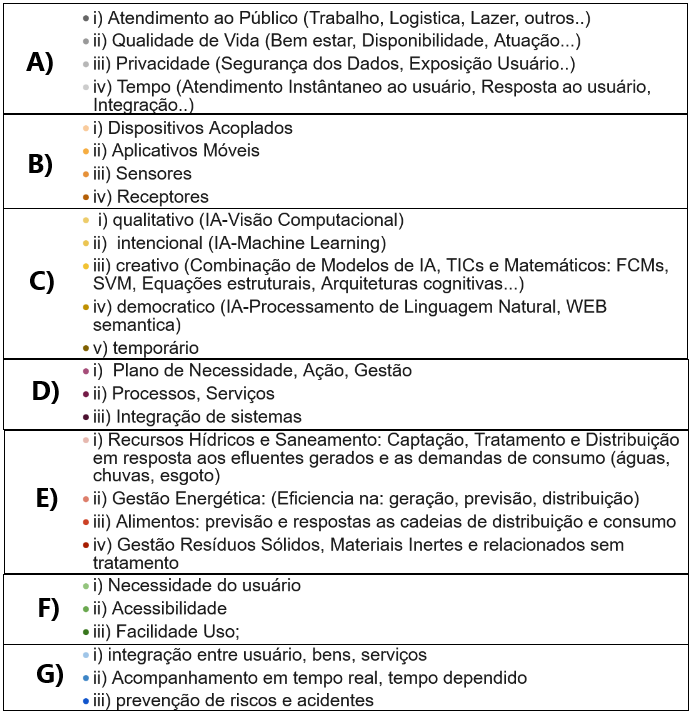
\includegraphics[width=0.85\textwidth,keepaspectratio]{images/FIGURA1_C.png}
        \caption{Atributos Categorizados.}
    
    \end{subfigure}

    \caption{\textit{Framework} com dimensões, domínios e atributos para cognição em cidades.}\label{fig-1}
    \source{\textcite{giuriatti2024}.}
\end{figure}

A estrutura (Figura \ref{fig-1}) descreve e classifica onze dimensões com destaque para as cinco principais: Infraestrutura; Gestão Pública; Mobilidade/Transportes; Sustentabilidade; e Segurança. Também, a estrutura compreende, dentre as dimensões, o envolvimento pela categorização dos elementos por sete domínios com seus respectivos atributos.

A formulação de uma estrutura \textit{``framework"} pode ser descrita como conjunto de classes que constitui um projeto abstrato para a solução de uma família de problemas \cite{fayad1999, johnson1988}; uma arquitetura desenvolvida com o objetivo de atingir a máxima reutilização, representada como um conjunto de classes abstratas e concretas, com grande potencial de especialização \cite{mattsson2000}; de atender a um conjunto de responsabilidades para uma aplicação específica ou um domínio de aplicação \cite{johnson1991, gamma1995}; um software parcialmente completo projetado para ser instanciado \cite{buschmann1996}.

Para analisar uma estrutura \textit{“framework”} quanto aos domínios que podem ser empregados, a proposição de uma ontologia é uma forma que os engenheiros do conhecimento possuem para entender o domínio, modificando e desenvolvendo a ontologia na direção de uma versão estável \cite{rautenberg2008}. Estas servem como ferramenta para organização, reuso e disseminação de conhecimento já especificado, facilitando a construção de novos agentes. Outrossim, para este tipo de solução, as ontologias desempenham um papel ainda mais importante como servir de vocabulário de comunicação entre agentes inteligentes \cite[p. 4]{freitas2004}.

A escolha do domínio e escopo da ontologia baseia-se nos princípios das escolhas que determinam os componentes desta \cite{campos2007}. Sendo as ontologias de domínio as quais versam especificamente sobre um domínio de conhecimento (medicina, automóveis etc.) \cite{almeida2013}.

Alguns requisitos para definição de uma ontologia são descritos por \textcite[p. 15]{freitas2004}, são eles:

\medskip
\begin{itemize}
    \item Por especificação explícita, podemos entender as definições de conceitos, instâncias, relações, restrições e axiomas.
    \item Por formalização, que é declarativamente definida, portanto, compreensível para agentes e sistemas.
    \item Por conceitualização, que se trata de um modelo abstrato de uma área de conhecimento ou de um universo limitado de discurso.
    \item Por compartilhamento, por tratar-se de um conhecimento consensual, seja uma terminologia comum da área modelada, ou acordada entre os desenvolvedores dos agentes que se comunicam.
\end{itemize}
\medskip

\textapud{martins2002}{Picker2007} afirma que a construção de uma ontologia requer o uso de um vocabulário específico para descrever uma realidade e mais um conjunto de axiomas lógicos necessários para dar semântica ao significado pretendido pelas palavras desse vocabulário. De acordo com a autora, deve se basear na utilização dos seguintes objetos:
 \medskip 
\begin{itemize}
    \item entidades, que descrevem conceitos (elementos de um domínio estudado) e providenciam uma representação lógica;
    \item atributos, que descrevem as propriedades das entidades;
    \item relações, que descrevem as ligações entre objetos no modelo (entidades e atributos);
    \item restrições, condições que o projetista impõe sobre as entidades, atributos ou relações.
\end{itemize}
 \medskip 
 
Considerando as dimensões no contexto \textit{smart campus} \cite{giuriatti2023} e das cidades que buscam a cognição \cite{giuriatti2024}, bem como considerando a evolução do ambiente \textit{smart} para o cognitivo descritos pelos autores supracitados e ao modelo estruturado para uma cidade cognitiva contendo as dimensões, os domínios e atributos evidenciados pela pesquisa \cite{giuriatti2024}, surge a definição do problema deste estudo: Como estruturar um modelo de campus para a cognição considerando uma dimensão específica, ``Infraestrutura", no contexto universitário? A partir dessa definição, é realizada uma revisão da literatura com os dados coletados dos artigos que contemplem modelos cognitivos no contexto universitário para enriquecimento da proposta deste estudo, e relacionar os elementos descritos nas pesquisas de \textcite{giuriatti2023, giuriatti2024}, sendo estruturados estes elementos por meio de um \textit{framework} e validados por ontologias com entidades, atributos, relações e restrições definidas por \textapud{martins2002}{Picker2007} e com seus requisitos especificados por \textcite{freitas2004}.

\section{Materiais e Métodos}
A metodologia da pesquisa constitui caráter exploratório, em uma abordagem qualitativa, por apresentar uma revisão integrativa sobre ferramentas e modelos; sintetizando os achados de estudos, transformando-os na construção de novas teorias \cite{whitemore2005} e por ter a finalidade de realizar uma análise do conhecimento pré-existente sobre os tópicos pesquisados \cite{russell2005}. Objetiva-se identificar as principais iniciativas que empregam modelos cognitivos no contexto universitário, e sua relação com a dimensão Infraestrutura para estruturação e concepção dos domínios e atributos no \textit{framework} proposto. Após, é demonstrada a proposta da ontologia com os critérios para definição das classes e subclasses, instâncias e propriedades do objeto pela ferramenta Protégé para validação do \textit{framework} proposto.

\subsection{Critérios de Inclusão de Trabalhos}
A exploração do termo ``Universidades Cognitivas" e ``modelos cognitivos" no contexto universitário foi realizada a partir da busca nas bases de dados Scopus, Web of Science e IEEE Xplore em ``títulos" de artigos publicados até março de 2024. Após, foi realizada a sobreposição dos artigos para retirada dos duplicados e daqueles obtidos no contexto dos modelos cognitivos que se aderem pela análise dos resumos ao contexto universitário. Os resultados dos registros aptos no contexto universitário com a identificação e retirada de registros fora do escopo da pesquisa – trabalhos que tratam sobre o comportamento cognitivo dos alunos universitários, como os de ordem comportamental, demência, depressão, dependências, drogas, ingresso, níveis de aprendizagem, neurológicas e outras – estão expostos na Figura \ref{fig-2}.

\begin{figure}[h!]
    \centering
    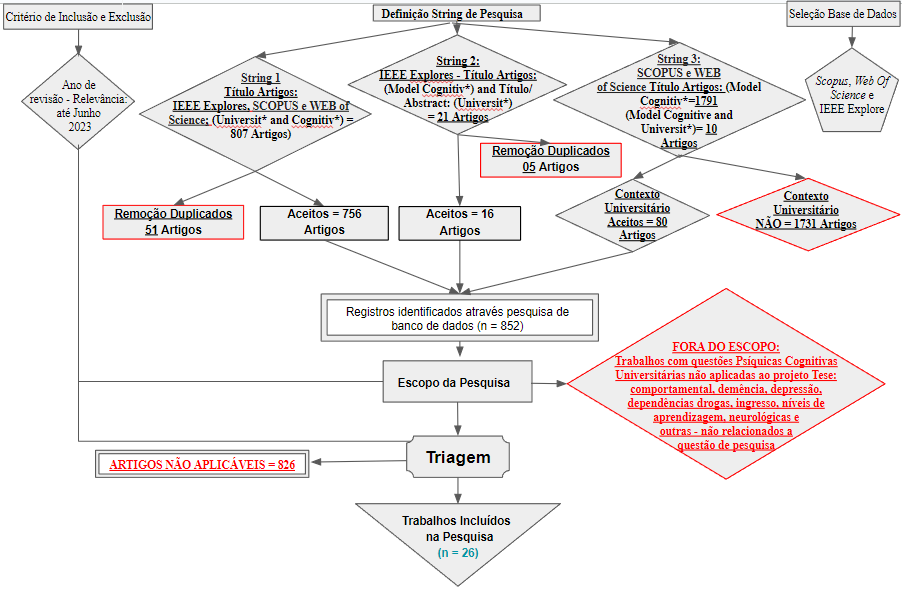
\includegraphics[width=\linewidth]{images/FIGURA2.png}
    \caption{Procedimentos de revisão do portfólio bibliográfico em Universidades Cognitivas.}
    \label{fig-2}
    \source{Elaborado pelos autores.}
\end{figure}

Com isso, conforme detalhamento da Figura \ref{fig-2} foram incluídos, após os critérios de análise do portfólio bibliográfico descritos nesta seção, um total de 26 artigos completos utilizados nesta pesquisa.

\subsection{Formulação do Framework Inicial}
Estes trabalhos, obtidos nos critérios de Inclusão de Trabalhos, são revisados e aglutinados aos atributos e domínios contidos no \textit{framework} \cite{giuriatti2024} para a posterior descrição do \textit{framework} proposto e instanciação na ferramenta Protégé na dimensão Infraestrutura.

\subsection{Definição das Ontologias para validação do Framework}

Utilizou-se o programa Protégé como ferramenta para elaboração da ontologia para representação dos domínios e as relações destes no contexto das demandas e atividades universitárias na dimensão específica definida em Infraestrutura. A definição das classes e construção das subclasses, instâncias e métricas de medição das relações entre estes termos basearam-se na revisão da literatura dos artigos (Figura \ref{fig-2}), e, na dimensão Infraestrutura, considerando os elementos que se relacionam com o contexto de um \textit{campus} contidos no modelo de \textcite{giuriatti2024}.

A definição das classes considerou o modelo abordado na ontologia de \textcite{rezaei2021}, onde as subclasses podem ser definidas para atendimento dos objetivos finais, neste caso, de uma Cidade Cognitiva, sendo replicável pelo objetivo desta pesquisa. Outro ponto, é que estas ontologias são um instrumento - nos moldes de uma cidade interconectada, desde a coleta de dados heterogêneos de sensores, dispositivos IoT e outras fontes de informação -, interligadas e integrando os dados coletados em uma plataforma complexa de forma que todos os serviços possam utilizar as informações geradas \cite{rezaei2021}.

Já a definição das métricas adotadas nas instâncias das ontologias na dimensão Infraestrutura considerou as entidades, atributos, relações e restrições apontadas por \textapud{martins2002}{Picker2007} e os objetivos de exercício de avaliação definidos por \textcite{mostashari2011}.

Por fim, a propriedade do objeto (ferramentas adotadas para a cognição de um campus) no programa Protégé, baseou-se nas relações que possuem os domínios e respectivos atributos categorizados por \textcite{giuriatti2024}, que relata a classificação e descrição dos modelos cognitivos aplicados no contexto das cidades com as respectivas ferramentas e tecnologias.

\section{Resultados e Discussão}

A partir da seleção dos trabalhos resgatados dos modelos cognitivos que abrangem os ambientes universitários (Figura \ref{fig-2}), é descrita a estruturação do \textit{framework} na dimensão Infraestrutura, baseada, em parte, na ideia inicial dos elementos categorizados por \textcite{giuriatti2024}, contidos na Figura \ref{fig-1}, e nos autores que serão contextualizados no decorrer das descrições das ontologias que fundamentaram o modelo proposto (Figura \ref{fig-3}).

\begin{figure}[h!]
    \centering
    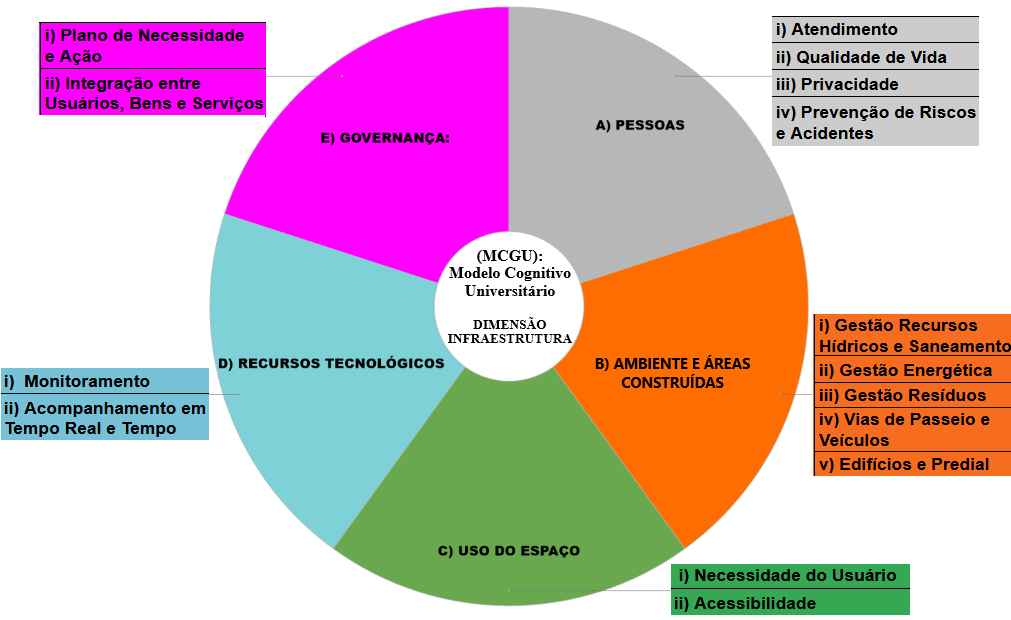
\includegraphics[width=0.90\linewidth]{images/FIGURA3.png}
    \caption{\textit{Framework} inicial Dimensão Infraestrutura em Universidades Cognitivas.}
    \label{fig-3}
    \source{Elaborado pelos autores.}
\end{figure}

O \textit{Framework} Inicial Dimensão Infraestrutura (Figura \ref{fig-3}) absorve os domínios dos Modelos Cognitivos das Cidades (Figura \ref{fig-1}) são eles: A) Pessoas e os respectivos atributos i) ao iii); domínio C) Uso do Espaço e os respectivos Atributos i) e ii); domínio E) Governança e os respectivos Atributos i) e ii). Também foram absorvidos alguns atributos relatados nos Modelos Cognitivos das Cidades (Figura \ref{fig-1}), são eles: Atributo i) Gestão de Recursos Hídricos e Saneamento, ii) Gestão Energética e iii) Gestão de Resíduos contidos no domínio E); o Atributo ii) Acompanhamento em Tempo Real e Tempo Dependido no domínio G). Os domínios B) Interação Humano Computador/Computação Cognitiva e C) Modelos Cognitivos, Conectivismo TICs e (IoT) em Dados, bem como, seus respectivos atributos relatados nos Modelos Cognitivos das Cidades (Figura \ref{fig-1}), são absorvidos como ferramentas para a cognição nos domínios traçados na dimensão infraestrutura pelas propriedades dos objetos (Figura \ref{fig-4}).

\begin{figure}[h!]
    \centering
    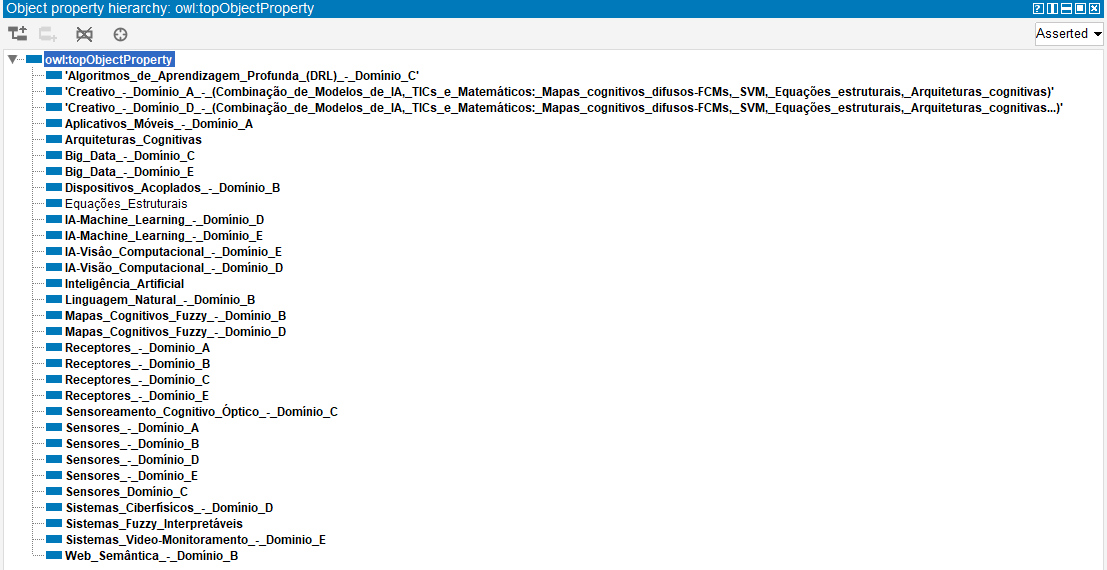
\includegraphics[width=0.90\linewidth]{images/FIGURA4.png}
    \caption{Definição das Propriedades dos Objetos – Ferramentas e Tecnologias aplicadas aos Domínios.}
    \label{fig-4}
    \source{Elaborado pelo autor na ferramenta Protégé.}
\end{figure}

A seguir, são demonstrados de forma visual as relações dos domínios com cada subclasses, instâncias, métricas e respectivas propriedades do objeto (ferramentas).

\begin{figure}[h!]
    \centering
    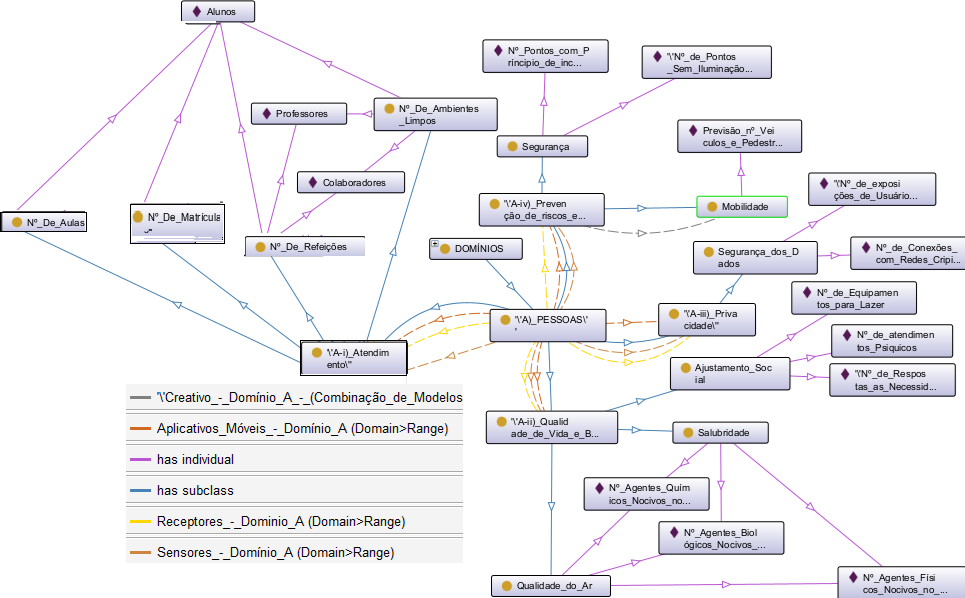
\includegraphics[width=0.95\linewidth]{images/FIGURA5.png}
    \caption{Visualização da Ontologia Infraestrutura no Domínio Pessoas.}
    \label{fig-5}
    \source{Elaborado pelo autor na ferramenta Protégé.}
\end{figure}
\bigskip
Na Ontologia Infraestrutura o Domínio A) Pessoas é descrito (Figura \ref{fig-5}) pelas subclasses: 
\medskip
\begin{itemize}
    \item i) \textit{Atendimento} com quatro métricas de medição: Nº de aulas, Nº de matrículas, Nº de refeições e Nº de ambientes limpos, sendo aplicados às instâncias alunos, colaboradores e professores. As ferramentas aplicadas são sensores, receptores e aplicativos móveis.
    \item ii) \textit{Qualidade de Vida e Bem-estar} é dirigida a três aplicações. Aplicação Ajustamento Social com três métricas de medição: Nº de Equipamentos para Lazer, Nº de Atendimentos Psíquicos e Nº de Respostas às Necessidades dos Usuários. As Aplicações Qualidade do Ar e Salubridade possuem as mesmas métricas, sendo três instâncias: Nº de Agentes Químicos Nocivos no Ambiente, Nº de Agentes Biológicos no Ambiente e Nº de Agentes Físicos Nocivos no Ambiente. Nesta subclasse as ferramentas aplicadas são sensores, receptores e aplicativos móveis.
    \item iii) \textit{Privacidade} possui uma aplicação na segurança de dados, sendo duas métricas de medição: Nº de exposições dos usuários e o Nº de Conexões com redes criptografadas. Nesta subclasse as ferramentas aplicadas são sensores, receptores e aplicativos móveis.
    \item iv) \textit{Prevenção de Riscos e Acidentes} possui aplicações em mobilidade e segurança. Sendo as métricas na segurança as instâncias: Nº de Pontos com Princípio de Incêndio e Nº de Pontos Sem Iluminação. A métrica em mobilidade é Nº de Veículos e Pedestres nas Vias de acesso do campus. Nesta subclasse tem-se para ambas as aplicações as ferramentas: sensores, receptores e aplicativos móveis. A aplicação mobilidade possui uma ferramenta a mais denominada ``Creativo": combinação de modelos IA, TICs, Matemáticos, Mapas Cognitivos Difusos (FCMs), SVM e outros.
\end{itemize}
\medskip

A cognição nas subclasses i), ii), iii) e iv) são formatadas pela utilização dos aplicativos móveis para uma comunicação multidirecional \cite{kaltenrieder2015}, possibilitando que todos os níveis da organização sejam incluídos e ouvidos \cite{bittenbinder2020} para o Atendimento ao aluno pela identificação do número de refeições, ambientes limpos, nº de aulas disponíveis. Compreende também a inserção de sensores e receptores constituídos por camadas \cite{chesnevar2020}, sendo uma camada física que pode ser desenvolvida por uma arquitetura cognitiva baseada por IA e Big Data \cite{park2019}, composta por ferramentas de software e hardware \cite{mansouri2018} para a integração da informação pela camada de dados \cite{khansari2015}. Essa estrutura de receptores e sensores conectados favorecem uma rede sustentável de tecnologias \cite{chapman2021} pela captação de dados oriundos dos aplicativos móveis nas instâncias das subclasses i, ii, iii e iv.

Na subclasse iv) a aplicação mobilidade é formatada pela complementação de uma estrutura denominada ``Creativo", que é a combinação de modelos IA, TICs, Matemáticos, Mapas Cognitivos Difusos (FCMs), SVM e outros. Sendo a utilização de mapas cognitivos difusos (FCMs) e SVM por meio de IA e modelos matemáticos uma forma de promover a tomada de decisão \cite{maio2015} no fluxo de veículos e pedestres na universidade, formatando uma proposta de um esquema dinâmico para prever os movimentos e desenvolver o gerenciamento eficiente por meio de subsistemas de imagem, biossensor, sensoriamento remoto e comunicação – TICs \cite{sastry2017}.

\begin{figure}[h!]
    \centering
    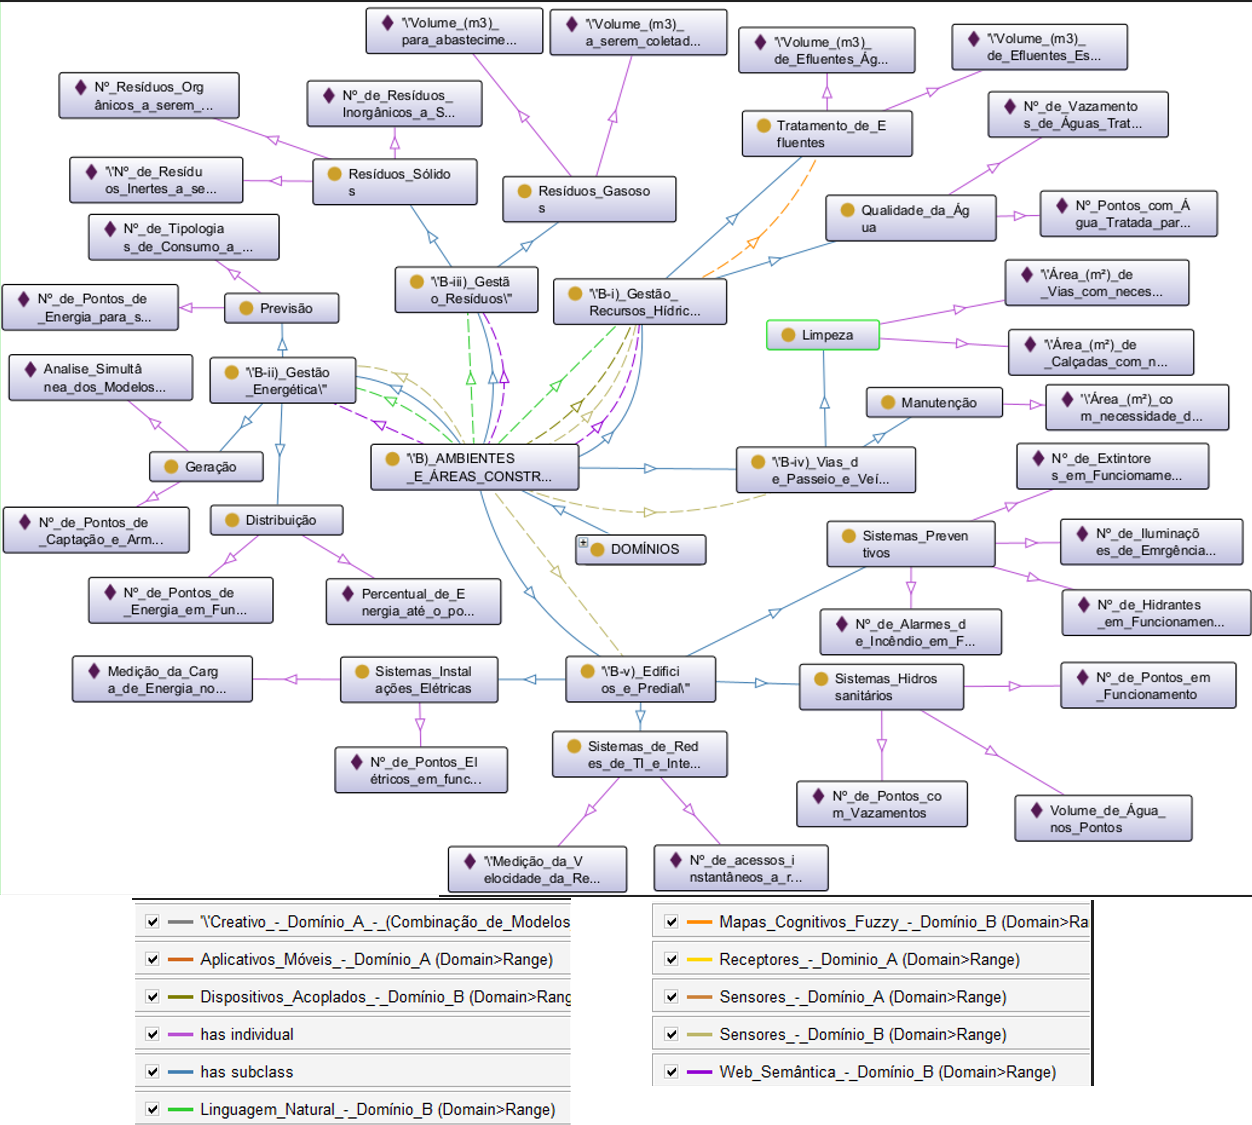
\includegraphics[width=0.95\linewidth]{images/FIGURA6.png}
    \caption{Visualização da Ontologia Infraestrutura no Domínio Ambiente e Áreas Construídas.}
    \label{fig-6}
    \source{Elaborado pelo autor na ferramenta Protégé.}
\end{figure}

Na Ontologia Infraestrutura o Domínio B) Ambiente e Áreas Construídas (Figura \ref{fig-6}) é descrito pelas subclasses:
\medskip
\begin{itemize}
    \item i) \textit{Gestão Recursos Hídricos e Saneamento} sendo dirigida por duas aplicações. Aplicação Tratamento de Efluentes contém duas métricas de medição: Volume de Efluentes de Esgoto ($m^3$) e Volume de Efluentes de Águas de Chuvas ($m^3$). As ferramentas aplicadas são sensores, mapas cognitivos \textit{fuzzy}, web semântica, dispositivos acoplados e linguagem natural. Já a Aplicação Qualidade da Água contém duas métricas de medição: Nº de Vazamentos de Águas Tratadas e Não Tratadas e Nº Pontos com Água Tratada para Consumo. As ferramentas aplicadas são sensores, web semântica, dispositivos acoplados e linguagem natural.
    \item ii) \textit{Gestão Energética} é dirigida a três aplicações. A aplicação Previsão com duas métricas: Nº de Pontos de Energia a Serem Atendidos e Nº de Tipologias de Consumo Atendidos no Ambiente. A aplicação Geração possui duas métricas: Análise Simultânea Dos Modelos Energéticos em Funcionamento e Nº de Pontos de Captação e Armazenamento em Funcionamento (ambas as métricas alimentadas por sistemas eólicos, solares e pelas redes de distribuição). A aplicação Distribuição possui duas métricas: Percentual de Energia até o ponto de Consumo e Nº de Pontos de Energia em Funcionamento. As ferramentas aplicadas são sensores, web semântica e linguagem natural.
    \item iii) \textit{Gestão de Resíduos} possui duas aplicações. Aplicação Resíduos Sólidos possui três métricas relacionadas ao volume de Resíduos ($m^3$): Resíduos orgânicos a serem coletados, Resíduos Inertes a serem coletados e Resíduos Inorgânicos a serem coletados. A aplicação Resíduos Gasosos possui duas métricas relacionadas ao volume de Resíduos ($m^3$): proveniente dos sistemas de esgotos existentes e abastecimento dos sistemas Prediais. As ferramentas aplicadas são web semântica, linguagem natural e sensores.
    \item iv) \textit{Vias de Passeio e Veículos} possui duas aplicações. Aplicação Manutenção definida pela métrica: Área ($m^2$) com necessidade de Reparos e Desobstrução. Na aplicação Limpeza a métrica é: Área ($m^2$) de calçadas com necessidade de Limpeza. As ferramentas aplicadas são os sensores.
    \item v) \textit{Edifícios e Predial} possui quatro aplicações. Aplicação Sistemas Hidrossanitários possui três métricas: Nº de pontos em Funcionamento, Nº de Pontos com Vazamentos e Volume de Água nos Pontos ($m^3$). A aplicação Sistemas de Redes de TI e Internet possui duas métricas: Nº de acessos instantâneos e Medição da Velocidade da Rede Internet (Mbps). A ferramenta aplicada são os sensores. A aplicação Sistemas Preventivos possui quatro métricas: Nº de Iluminação de Emergência em Funcionamento, Nº de Alarmes de Incêndio em Funcionamento, Nº de Extintores em Funcionamento e Nº de Hidrantes em Funcionamento. A ferramenta aplicada são os sensores. A aplicação Sistemas de Instalações Elétricas possui duas métricas: Nº de pontos de tomadas e iluminação em Funcionamento e Medição de Carga de Energia nos pontos Tomadas e Iluminação em Funcionamento.
\end{itemize}
\medskip

A cognição nas subclasses i), ii), iii), iv) e v) são formatadas por sensores para a confiabilidade e eficiência por meio de algoritmos e \textit{blockchain} que selecionam os nós dos sensores com melhor desempenho \cite{rani2022} e realizam a captação dos dados em vários pontos do \textit{campus} para melhoria de serviços (por ex: de luz, ventilação de ar condicionado, métodos de segurança para plantas de energia), identificando o risco operacional quando a ferramenta cognitiva está vinculada ao diagnóstico preditivo dos dados captados nos sensores de vários dispositivos por uma camada IoT, fornecendo os dados para o modelo de computação cognitiva, desempenho do equipamento e sua flexibilidade na perspectiva de tempo real \cite{daniel2021} por uma estrutura de ponta em nós \cite{rausch2021}. Nas subclasses a captação por sensores em redes sem fio favorecem a cognição pela definição, escalação e resposta nas atividades e ações \cite{daniel2021} e integração dinâmica na análise e processamento de dados por um servidor \cite{patra2017}, obtidos pelas métricas e instâncias projetadas. Na classe iv), a utilização de sensores promove o monitoramento de objetos e diferentes contextos nas vias públicas com resposta ao contexto \cite{somov2013, singh2014}. A cognição por receptores nas subclasses é aplicável pelo rastreamento dos dados \cite{rausch2021} identificando indivíduos e objetos num raio de 100 $m$ obtendo suas posições e o rótulo da classe do objeto, onde são contabilizados os dados e informações por vários computadores de ponta, bem como câmeras e outros sensores interligados entre si através de um \textit{middleware} de mensagens \cite{rausch2021}. Outra forma de aplicação por receptores é na subclasse da gestão energética, especificamente usando a técnica de comutação de antena em conjunto ao rádio cognitivo e acesso múltiplo não ortogonal (NOMA) \cite{alzahrani2018} para avaliar o sistema de previsão, geração e distribuição de energia no campus.

Nas subclasses i), ii) e iii), a utilização da linguagem natural favorece a cognição por gerenciar a incerteza na coleta dos dados, trazendo significado e padrões de resposta \cite{hudec2019}, processando informações pela interação entre pessoas e campus e entre pessoas e pessoas \cite{donofrio2018}, em que a informação transmitida por uma instância ou subclasse seja compilada, levando a uma melhor representação de uma realidade complexa, sendo mais claras de ler e entender para posterior manipulação e atualizações em tempo hábil \cite{tabacchi2019} e possibilitando que usuários examinem os elementos do mecanismo de inferência simplesmente lendo essas informações \cite{alonso2018}. A Web Semântica é aplicada nas subclasses i), ii) e iii) como uma forma da cognição para vencer o desafio das aplicações por redes de sensores na coleta de dados heterogêneos usados em diferentes aplicações \cite{LimaTeran2019}, trazendo significado aos dados \cite{cuenca2018}, podendo ser estruturada na subclasse pela linguagem natural e analisadas pela Web Semântica \cite{park2019, karasan2021}.

Os dispositivos acoplados aplicados na subclasse i) promovem a cognição pela conexão destes com os sistemas controlados por internet e web \cite{donofrio2018}, sendo conectados a um meio físico como forma de coletar e armazenar os dados a serem transmitidos por sensores \cite{rausch2021}. Isso possibilita o controle do volume de efluentes gerados e o seu tratamento, de vazamentos pela entrada de água nas tubulações e sua saída nos pontos de uso no campus, com armazenamento destes dados, para posterior transmissão por sensores até uma central de dados. São identificados os dados transmitidos e analisados por Web Semântica, que utiliza a informação recebida para construir modelos semânticos, facilitar quais estados e automações do raciocínio físico e semântico \cite{park2019}.

\begin{figure}[h!]
    \centering
    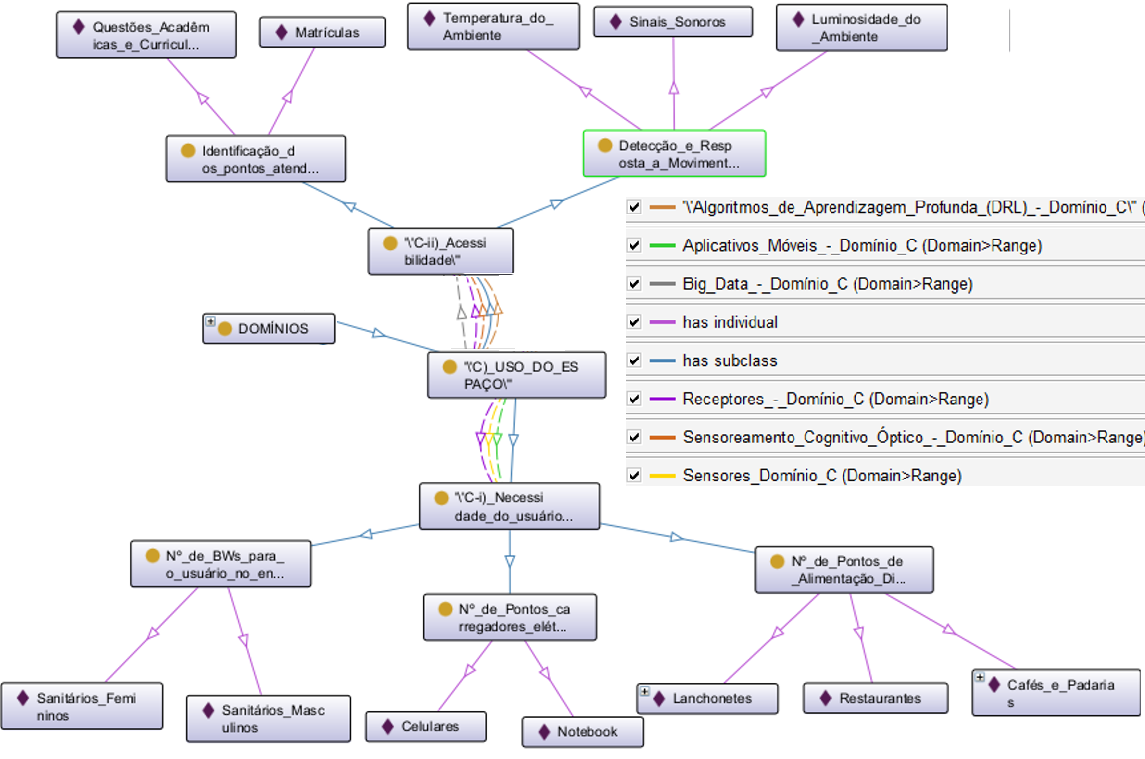
\includegraphics[width=0.90\linewidth]{images/FIGURA7_1.png}
    \caption{Visualização da Ontologia Infraestrutura no Domínio Uso do Espaço.}
    \label{fig-7}
    \source{Elaborado pelo autor na ferramenta Protégé.}
\end{figure}

Na Ontologia Infraestrutura o Domínio C) Uso do Espaço (Figura \ref{fig-7}) é descrito pelas subclasses:

\medskip
\begin{itemize}
\item i) \textit{Necessidade do Usuário} possui três métricas para medição: Nº de BWCs para o usuário no entorno Disponíveis ao Uso, Nº de Pontos de carregadores elétricos disponíveis ao uso e Nº de Pontos de Alimentação Disponíveis. A métrica Nº de BWCs para o usuário aplicadas as instâncias Sanitários Uso Feminino e Uso Masculino. A métrica Nº de Pontos de carregadores elétricos são aplicados às instâncias Celulares e Notebooks. Por fim, a métrica Nº de Pontos de Alimentação Disponíveis são aplicadas as instâncias Lanchonetes, Restaurantes, Cafés e Padarias dentro e nas imediações do \textit{campus}. As ferramentas aplicadas são sensores, receptores e aplicativos móveis.
\item ii) \textit{Acessibilidade} é dirigida a duas aplicações. A aplicação Identificação dos Pontos de Atendimento aos Alunos possui duas métricas: Questões acadêmicas (gestão das necessidades que demandam respostas por servidores, colaboradores e professores no âmbito da formação acadêmica) e Curriculares e Matrículas (que cabem interação com gestores e colaboradores quanto a instrução dos alunos nos processos de escolhas de disciplinas na formação acadêmica e profissional). A aplicação Detecção e Resposta aos Movimentos dos Alunos possui três métricas: Temperatura do Ambiente (conforto e climatização que favoreçam o bem-estar e aprendizado do aluno no ambiente). A métrica Sinais Sonoros busca dar resposta a questões de perigo no ambiente (como riscos de: incêndio, vazamentos de gases, choque elétrico, atitudes suspeitas de pessoas que coloquem em risco a vida no ambiente acadêmico). Por fim, a métrica luminosidade do ambiente traz uma forma de propor o conforto e segurança no trânsito do campus como corredores, salas de aulas e bibliotecas, que proponham ao aluno o aprendizado de forma eficiente pelo índice de luminosidade apropriado. As ferramentas aplicadas são sensores cognitivos ópticos, algoritmos de aprendizagem profunda (DRL), receptores e Big Data. Algumas questões como a definição da localização e disponibilidade são conduzidas por aplicativos para a localização dos equipamentos e pontos na zona do usuário (estudantes, professores, colaboradores e público externo) por meio da camada de percepção \textit{(Reader)} de \textit{Bluetooth} e \textit{Mobile Phone} (Rede) \cite{fang2018}. 
\end{itemize}
\medskip

Os receptores aplicados para a cognição nas subclasses i) e ii) são constituídos por uma camada de serviços com arquitetura cognitiva \cite{park2019} para atender às questões acadêmicas dos estudantes, do ambiente de estudos com detecção e resposta a movimentos dos estudantes e usuários, aos pontos de uso dos equipamentos e pontos de alimentação e carga de dispositivos elétricos. Sendo compostos por ferramentas de \textit{Software} e \textit{Hardware} \cite{mansouri2018} para a integração da informação pela camada de dados \cite{khansari2015}. Essa estrutura de receptores em conjunto aos sensores conectados e aplicativos móveis nas instâncias da ontologia da subclasse i) favorecem sua estruturação pela captação de uma rede sustentável de tecnologias \cite{chapman2021}.

A utilização dos algoritmos de aprendizagem profunda supervisionada (DRL) torna cognitiva a subclasse ii), por promover o atendimento aos estudantes, ao aprenderem com os dados gerados \cite{mohammadi2018}, em questões referentes às matrículas geradas para ações de direcionamento dos estudantes no meio acadêmico. Bem como, a detecção e resposta (temperatura, sinais sonoros e luminosidade) aos movimentos são facilitadores de serviços cognitivos, como agentes de aprendizagem que evoluem conforme as condições da mudança ambiental e executa funções e ações autônomas sem intervenção humana, por meio de objetos virtuais inteligentes em serviços de cidades inteligentes, em conjunto com algoritmos DRL, onde esses objetos podem aprender, decidir e agir de forma autônoma \cite{mohammadi2018}.

A aplicação da cognição para identificação dos pontos de atendimento dos estudantes e utilização dos ambientes pela detecção e resposta aos movimentos dos estudantes e usuários na subclasse ii) é realizada por Big Data e por algoritmos de aprendizagem \cite{wang2023}. Sendo o Big Data uma forma, nesta aplicação da subclasse, para compreender os comportamentos de indivíduos e grupos \cite{sangwan2021}, analisando o agrupamento e localização de indivíduos e objetos apontados por \cite{coccoli2022}, especificamente neste caso, dos estudantes pela identificação dos consumos de energia e água em ambientes do campus como sala de informática, salão de bilhar do campus e outros locais de entretenimento, que são consumos em locais não essenciais, mas uma espécie de alto consumo específico \cite{wang2023}.

\begin{figure}[h!]
    \centering
    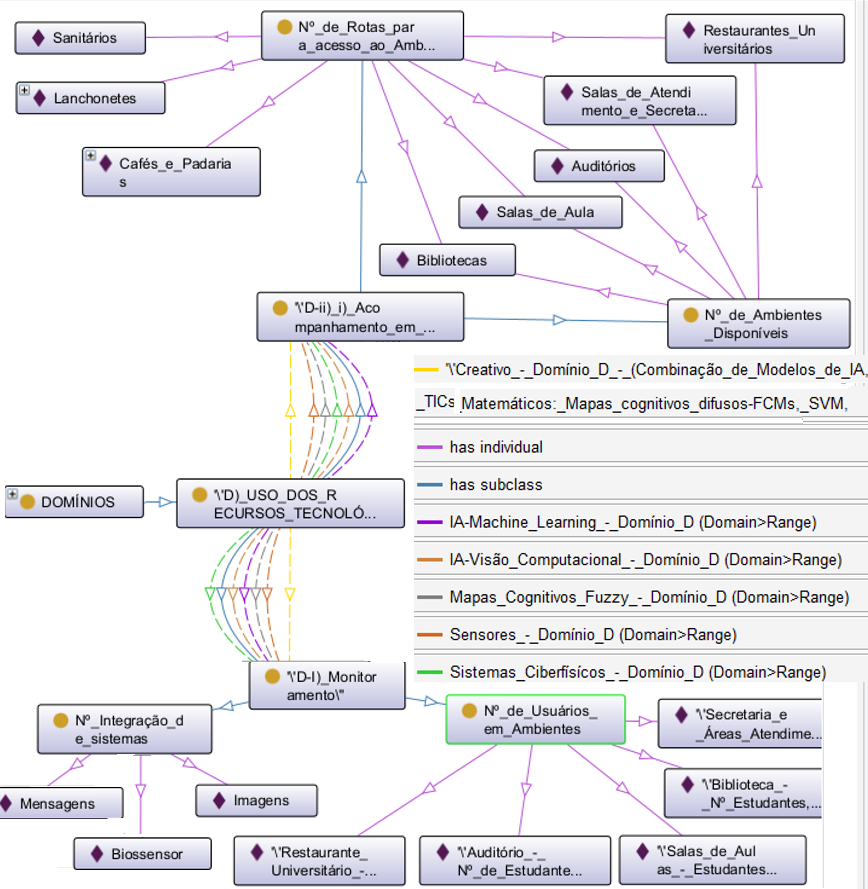
\includegraphics[width=0.90\linewidth]{images/FIGURA8.png}
    \caption{Visualização da Ontologia Infraestrutura no Domínio Uso Dos Recursos Tecnológicos.}
    \label{fig-8}
    \source{Elaborado pelo autor na ferramenta Protégé.}
\end{figure}
\bigskip
Na Ontologia Infraestrutura o Domínio D) Uso Dos Recursos Tecnológicos (Figura \ref{fig-8}) é descrito pelas subclasses:

\medskip
\begin{itemize}
\item i) \textit{Monitoramento} possui duas métricas: Nº de usuários em Ambientes (capacidade de sistemas e redes de internet para atendimento aos usuários) nas instâncias de atendimento em Restaurante Universitário, Bibliotecas, Auditórios, Salas de Aulas e Salas de Atendimento aos alunos vinculadas a Secretarias de atendimento aos estudantes. A segunda é Nº de Sistemas Integrados (atendimento as demandas dos usuários em tempo real) relacionados às instâncias de mensagens, imagens e biossensor.
\item ii) \textit{Acompanhamento em Tempo Real e Tempo despendido} possui duas métricas para medição: Nº Ambientes Disponíveis (relacionado a capacidade de resposta aos usuários) nas instâncias dos ambientes Restaurante Universitário, Bibliotecas, Auditórios, Salas de Aulas e Salas de Atendimento aos alunos vinculadas a setores. A segunda é Nº de Rotas para Acesso ao Ambiente (Relacionado aos deslocamentos dos alunos para um local onde há uma rota que é favorável o acesso de forma segura, ágil e sem obstruções). São aplicáveis nas instâncias Restaurante Universitário, Sanitários, Bibliotecas, Auditórios, Salas de Aulas e Salas de Atendimento aos alunos vinculadas a setores; e nos ambientes externos no entorno ao campus relacionados a cafés, padarias e lanchonetes. As ferramentas aplicadas são: Sensores, \textit{IA-Machine Learning}, IA-Visão Computacional, Mapas Cognitivos \textit{Fuzzy}, Sistemas Ciberfisícos e Creativo, que é a combinação de modelos IA, TICs, Matemáticos, Mapas Cognitivos Difusos (FCMs), SVM e outros. 
\end{itemize}
\medskip

A utilização de sensores nas subclasses i) e ii) torna cognitivo o campus pela aderência às questões de acompanhamento em tempo real e monitoramento dos recursos tecnológicos empregados em termos de resposta \cite{somov2013, singh2014, daniel2021}, adaptado ao contexto universitário relacionado ao nº de rotas de acesso, nº de usuários nos ambientes e nº de ambiente disponíveis.

A utilização de \textit{IA-Machine Learning} torna cognitiva as subclasses i) e ii) por desenvolver um ambiente que permite que o sistema aprenda com os dados e, portanto, o desempenho dos algoritmos de aprendizado desenvolve o reconhecimento de padrões \cite{sangwan2021}, promovendo a gestão dos ambientes do campus por algoritmos \cite{wang2023} nas subclasses i) e ii) pela análise do agrupamento dos estudantes na identificação dos consumos, por exemplo, dos ambientes de sala de informática do \textit{campus}, auditórios, restaurantes, cafés e lanchonetes do \textit{campus}, salas de aulas, bibliotecas e outros. Os mapas \textit{fuzzy} tornam cognitivos os ambientes do \textit{campus} nas subclasses i) e ii) pelos multicritérios apontados como essenciais para revelar a priorização das alternativas \cite{karasan2021}, sendo definidos pela ontologia por: nº de rotas por acessos ao ambiente, nº de ambientes disponíveis, nº de usuários no ambiente e nº de integração e sistemas disponíveis. Ressalta-se as grandes quantidades de dados interconectados \cite{donofrio2018} e as incertezas dos dados e informações recebidos \cite{tabacchi2019} para a tomada de decisão \cite{vaz2022}, relacionados ao âmbito dos recursos tecnológicos aplicados nos diferentes ambientes definidos pela ontologia.

Nas subclasses i) e ii) a aplicação da cognição pela complementação de uma estrutura denominada ``Creativo" é uma forma de análise quanto ao fluxo de estudantes, professores e usuários no \textit{campus}, podendo ser agrupados e analisados por algoritmos \cite{wang2023}, como proposta de um esquema dinâmico para integração de sistemas de mensagens, biossensor, imagens \cite{sastry2017} no gerenciamento eficiente do tráfego interno dos usuários nos ambientes onde todos os outros sistemas são notificados \cite{rezaei2021} quanto ao nº de rotas por acessos ao ambiente, nº de ambientes disponíveis e nº de usuários no ambiente. A utilização de sistemas ciberfísicos nas subclasses i) e ii) favorecem a cognição como papel importante no armazenamento dos dados e informações sensíveis ao contexto \cite{rahman2019}, com a garantia da segurança e da privacidade dos dados obtidos, sendo alcançados pelo monitoramento contínuo em sistemas \cite{machin2021}.

\begin{figure}[h!]
    \centering
    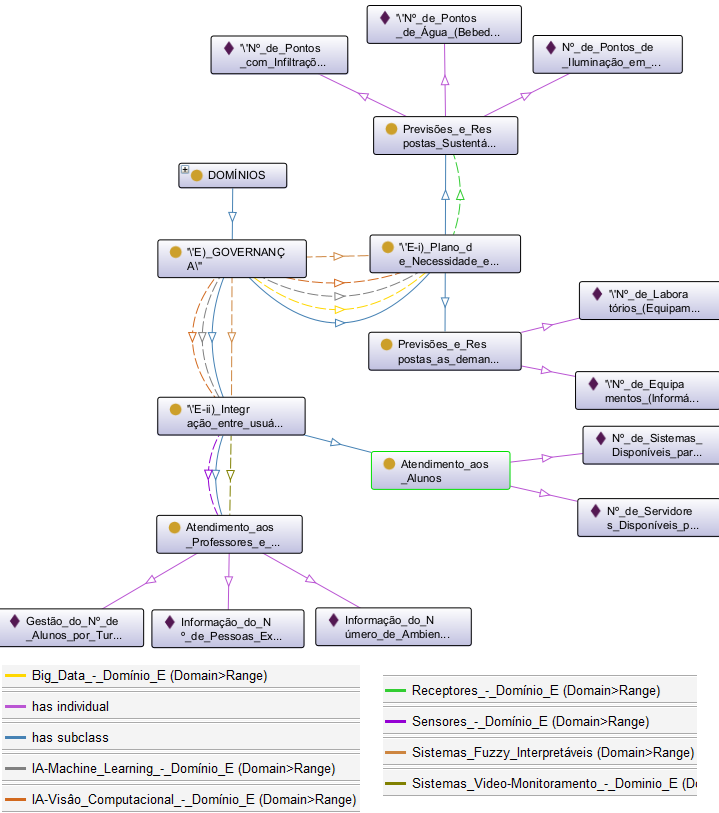
\includegraphics[width=0.90\linewidth]{images/FIGURA9.png}
    \caption{Visualização da Ontologia Infraestrutura no Domínio Governança.}
    \label{fig-9}
    \source{Elaborado pelo autor na ferramenta Protégé.}
\end{figure}

Na Ontologia Infraestrutura o Domínio E) Governança (Figura \ref{fig-9}) é descrito pelas subclasses:

\medskip
\begin{itemize}
\item i) \textit{Previsões e Respostas Sustentáveis} são formuladas três métricas: Nº de Pontos de Iluminação em Funcionamento (em ambientes como Restaurante Universitário, Biblioteca, Auditórios, Salas de Aulas e Salas de Atendimento aos alunos vinculadas a Secretarias e BWCs); Nº de Pontos de Água – Bebedouros (para atendimento as demandas dos usuários do \textit{campus}); Nº de Pontos com infiltrações (em ambientes como Restaurante Universitário, Biblioteca, Auditórios, Salas de Aulas e Salas de Atendimento aos alunos vinculadas a Secretarias e BWCs). São aplicadas nesta subclasse as ferramentas: Sensores, IA-\textit{Machine Learning}, IA-Visão Computacional, Sistemas \textit{Fuzzy} Interpretáveis, Big Data e Receptores. Na aplicação Previsões e Respostas as Demandas Acadêmicas são formuladas duas métricas: Nº de Laboratórios - Equipamentos Disponíveis (em ambientes como por exemplo Medicina Humana, Veterinária, Química, Biologia e outros que necessitem de resposta aos espaços e equipamentos disponíveis para estudos e ensaios); a segunda é Equipamentos Disponíveis para Uso (Informática) nos ambientes para alunos e colaboradores em locais como Biblioteca, Auditórios, Salas de Aulas, Laboratórios de Informática e Salas de Atendimento aos alunos vinculadas a Secretarias). São aplicadas as ferramentas nesta subclasse: Sensores, IA-\textit{Machine Learning}, IA-Visão Computacional, Sistemas \textit{Fuzzy} Interpretáveis, Big Data.
\item ii) \textit{Integração entre Usuários, Bens e Serviços} contém duas aplicações. A primeira é a aplicação Atendimento aos Alunos, para as quais são formuladas duas métricas: Nº de servidores disponíveis para atendimento as questões curriculares (onde o aluno obtém a informação específica de quem pode resolver as questões relacionadas as suas atividades acadêmicas no decorrer de sua formação); e Nº de sistemas disponíveis para as atividades acadêmicas a serem realizadas (onde o aluno obtém a informação dos meios, como programas, sistemas, softwares, e-mails e outros, acessíveis para a resolução de suas questões. A segunda aplicação é Atendimento aos Professores e Colaboradores, para a qual são formulados três métricas: Nº de pessoas Externas no Ambiente Universitário (para dimensionamento, por exemplo, do número de pessoas que irão frequentar ambientes do \textit{campus}), sendo uma forma de evitar possíveis conflitos relacionados aos acessos a ambientes restritos a alunos, professores, bem como por questões de segurança do meio universitário; Nº de Ambientes no Campus Disponíveis para Uso (Informa aos usuários do campus os locais que possuem acesso livre para um público específico, evitando questões de falta de disponibilidade para um uso específico, bem como a conflitos quanto ao uso e a segurança); e Nº de Alunos que Acessam o Campus (uma informação útil aos professores e colabores que precisam dimensionar, por exemplo, o início das aulas, as demandas de atendimentos presenciais, demandas de: limpeza, alimentação, acessos a internet e outros pertinentes as demandas de atendimento cotidiano no campus). São aplicadas nesta subclasse as ferramentas: IA-\textit{Machine Learning}, IA-Visão Computacional, Sistemas \textit{Fuzzy} Interpretáveis e Big Data. Nesta subclasse ii) a aplicação Atendimento aos Professores e Colaboradores possui além das ferramentas mencionadas acima o acréscimo dos sensores e sistemas de videomonitoramento.
\end{itemize}
\medskip

A utilização de sensores nas subclasses i) e ii) torna cognitivo o campus na subclasse Plano de Necessidade e Ação, aplicado nas questões de previsões das demandas acadêmicas e previsões nas respostas sustentáveis para aperfeiçoar o reconhecimento de padrões \cite{vaca-cardenas2020}, onde os dados dos sensores fornecem resultados para os serviços de IA com uso intensivo de computação \cite{rausch2021}, definindo, a partir destes dados, os cenários e descrevendo o comportamento e estado do ambiente com a(s) alternativa(s) de resposta para cada um desses cenários \cite{mostashari2011}. A utilização de IA-\textit{Machine Learning} é aplicável para tornar cognitiva as subclasses i) e ii), pois os algoritmos de aprendizado desenvolvem o reconhecimento de padrões \cite{sangwan2021} gerindo os ambientes do \textit{campus} por algoritmos \cite{wang2023}. Ao analisar os dados por agrupamento dos estudantes, professores e colaboradores, é identificado o número de equipamentos para uso nos ambientes. A aplicação de IA-\textit{Machine Learning} e sensores em conjunto nas subclasses i) e ii) favorecem uma arquitetura e desenvolvimento de uma rede cognitiva \cite{daniel2021}. A soma de IA-Visão Computacional e IA-\textit{Machine Learning} promove a cognição nas subclasses i) e ii), formando uma computação cognitiva no \textit{campus} que é composta por técnicas automáticas de aprendizado de máquina, que usam análise de dados, reconhecimento de padrões e processamento de linguagem natural para pensar como os humanos, quando treinados, não requerem assistência \cite{rahman2019}. A utilização de Sistemas de Videomonitoramento torna um campus cognitivo na subclasse ii) no atendimento aos professores e colaboradores, pela análise e gestão de indivíduos \cite{baig2018cognitive}, identificando possíveis ameaças \cite{kienzle2016} classificando, alertando e avisando os operadores por meio de informações e fotos \cite{coccoli2022}. A aplicação da cognição por Big Data nas Previsões e Respostas Sustentáveis e respostas às demandas acadêmicas na subclasse i), é realizada por algoritmos de aprendizagem \cite{wang2023} que faz a gestão dos dados dos ambientes a fim de organizá-los \cite{daniel2021}, identificando locais que possuem necessidade de assistência referentes aos equipamentos disponíveis, pontos de iluminação e água para o funcionamento pleno do ambiente. A utilização de receptores para a cognição na subclasse i), Previsão e Respostas Sustentáveis, atua como forma de receber as informações captadas por sensores quanto aos pontos que estão danificados, favorecendo a estruturação de uma rede sustentável de tecnologias \cite{chapman2021} que respondam às demandas dos ambientes nestas instâncias de subclasse, por meio de um \textit{middleware} de mensagens \cite{rausch2021}. Os sistemas \textit{fuzzy} interpretáveis aplicados para a cognição na subclasse i) desenvolvem o papel de transformar os dados coletados e transmitidos por sensores e receptores em informações interpretáveis, facilitando a interação e resposta \cite{alonso2018} e representando explicitamente a incerteza \cite{donofrio2018} nas demandas de previsões e resposta do ambiente a serem verificadas pelas instâncias desta subclasse.

Após a definição das ontologias por domínios é demonstrada a ontologia final, que demonstra os domínios (classes) categorizados de A) a E) e suas respectivas subclasses, além de demonstrar todas as ferramentas aplicadas nos domínios, classes e subclasses na Dimensão Infraestrutura (Figura \ref{fig-10}).

\begin{figure}[h!]
    \centering
    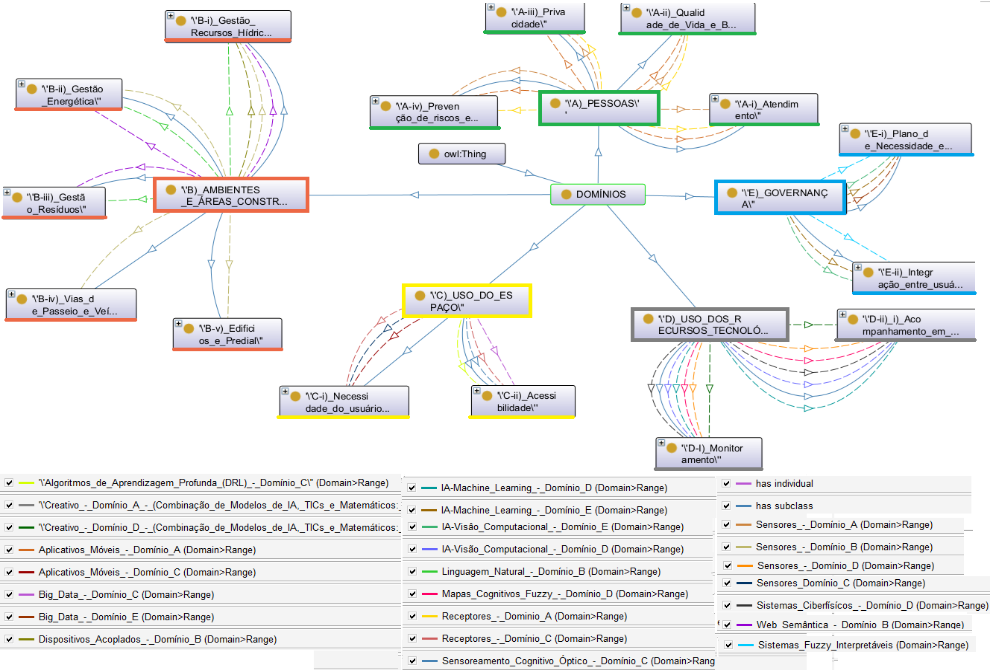
\includegraphics[width=0.95\linewidth]{images/FIGURA10.png}
    \caption{Ontologia da Dimensão Infraestrutura Final.}
    \label{fig-10}
    \source{Elaborado pelo autor na ferramenta Protégé.}
\end{figure}

\section{Conclusão}

Considera-se válida, para os fins do presente trabalho, a definição dos domínios e dos atributos obtidos no contexto dos modelos cognitivos empregados nas cidades por \cite{giuriatti2024}, pois contribuiu para delinear o \textit{framework} proposto.

Considerando a gama de dimensões contidas no contexto das cidades, a definição de uma dimensão específica, Infraestrutura, direcionou a aplicabilidade do \textit{framework} no contexto dos campi universitários, cujos domínios agrupados foram: Pessoas, Ambientes e Áreas Construídas, Uso do Espaço, Recursos Tecnológicos e Governança. Trata-se de uma base teórica e metodológica que possibilita a formatação da estrutura do \textit{framework}.

A utilização da ferramenta Protégé se mostrou válida para a construção de ontologias, sendo de grande valia para o cadastramento das propriedades do objeto (ferramentas) que foram utilizadas nas ontologias de cada domínio categorizados para a dimensão Infraestrutura.

Os domínios definidos e atributos categorizados que formularam o modelo da estrutura do \textit{framework} proposto são uma demonstração da aplicabilidade de cada domínio definido para a cognição de um \textit{campus} na dimensão proposta. Dentre os domínios, sensores, receptores e IA são as ferramentas com maior evidência dentre as ontologias demonstradas neste estudo para a cognição de um \textit{campus} na dimensão Infraestrutura.

Espera-se que futuros estudos possam aprofundar o tema desta pesquisa nas outras dimensões relativas a um \textit{campus} universitário, nos moldes das cidades cognitivas \cite{giuriatti2024}; como a estruturação de \textit{frameworks} que atendam as dimensões da sustentabilidade, segurança, gestão pública, saúde, educação, economia e finanças, mobilidade e transporte, meio ambiente e clima e social no contexto universitário.

Uma segunda linha de proposta de estudo futuro poderia abordar a adoção dos conceitos, atributos e métricas definidas nas ontologias com adoção e medição nos campi e avaliações constantes por pesquisadores que busquem transformar a ideia proposta na formulação do \textit{framework} numa proposta que atenda às situações e necessidades impostas pelas demandas e deficiências que podem ser vencidas com uso da implantação das ontologias.

Uma terceira linha seria desenvolver um conceito claro e aplicável de forma objetiva aos anseios dos campi, podendo ser realizadas pesquisas com gestores, diretores, servidores e pesquisadores dos campi quanto às necessidades e demandas a serem atendidas, para então desenvolver um modelo cognitivo adaptado e que atendam às especificidades de um \textit{campus}.


\printbibliography\label{sec-bib}
% if the text is not in Portuguese, it might be necessary to use the code below instead to print the correct ABNT abbreviations [s.n.], [s.l.]
%\begin{portuguese}
%\printbibliography[title={Bibliography}]
%\end{portuguese}


%full list: conceptualization,datacuration,formalanalysis,funding,investigation,methodology,projadm,resources,software,supervision,validation,visualization,writing,review
\begin{contributors}[sec-contributors]
\authorcontribution{Tiago Giuriatti}[conceptualization,methodology,formalanalysis,visualization,writing,review]
\authorcontribution{João Artur de Souza}[supervision,validation]
\authorcontribution{Gilberto Luiz de Souza Paula}[supervision,validation]
\authorcontribution{Chirley de Miranda Giuriatti}
[review]
\end{contributors}



\end{document}

